\linespread{1.5}
%use \usepackage{float}
\textbf{Solução}
    
\textbf{a)}
\begin{figure}[H]
    \centering
    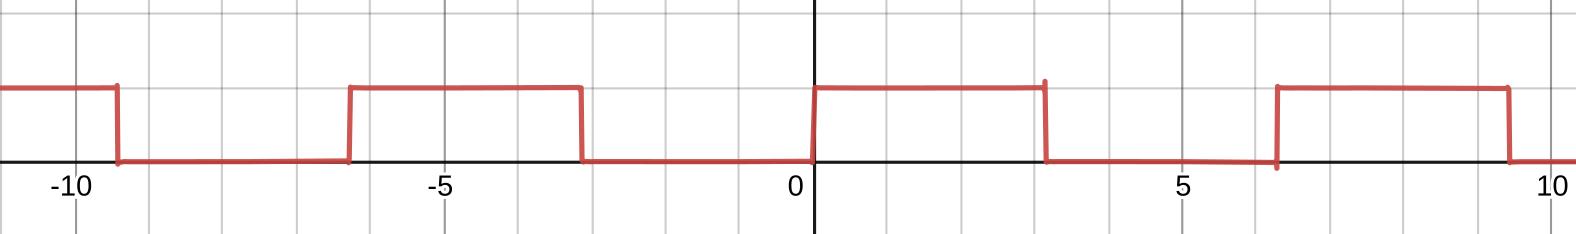
\includegraphics[width = 0.7\linewidth]{fig/sf4a.png}
    \caption{Como foi feita pelo site \textit{https://www.desmos.com/calculator} foi necessário limitar a série, o que permite ver os efeitos causados pela aproximação da série. Além disso no seu desenho deve mostrar os pontos que pertencem ou não aquela parte do gráfico, por exemplo: $-\pi \in y=0$, mas não pertence a $y=1$, os saltos de uma função pra outra também não existem de fato na função.}
\end{figure}

\textbf{b)}

Dada a equação que define a série de Fourier real:
\begin{equation}
    \label{eq:Fourierserie}
    f(t) = a_0 + \sum_{k=1}^\infty a_k\cos{(kwt)} + b_k\sin{(kwt)}
\end{equation}

E analisando a função $f(x)$, cujo período fundamental é $T=2\pi \xrightarrow{} w=1$, vemos que ela não apresenta nenhuma relação de paridade, portanto se faz necessário calcular todos os coeficientes de Fourier:
\begin{equation*}
    a_0 = \frac{1}{2\pi}\int_{-\pi}^\pi f(x)dx = \frac{1}{2\pi} \left( \int_{-\pi}^0 0dx + \int_0^\pi 1dx \right) = \frac{1}{2\pi}[x]_0^\pi
\end{equation*}
\begin{equation}
    \label{eq:sf4ba0}
    a_0 = \frac{1}{2}
\end{equation}

\begin{equation*}
    a_k = \frac{2}{2\pi}\int_{-\pi}^\pi f(x)\cos{(kwx)}dx = \frac{1}{\pi}\left(\int_{-\pi}^0\cos{(kwx)} 0dx + \int_0^\pi 1\cos{(kwtx}dx\right) = \frac{1}{\pi}\left[\frac{\sin{(kwx)}}{kw}\right]^\pi_0
\end{equation*}
\begin{equation}
    a_k = \frac{\sin{(k\pi)}}{k\pi}
\end{equation}

Como $k \in \N$ e $k\geq1$, então $\sin{(k\pi)}=0$, logo:

\begin{equation}
    \label{eq:sf4bak}
    a_k = 0
\end{equation}

\begin{equation*}
    b_k = \frac{1}{\pi}\int_{-\pi}^\pi f(x)\sin{(kwx)}dx = \frac{1}{\pi}\left(\int_{-\pi}^0\sin{(kwx)} 0dx + \int_0^\pi 1\sin{(kwtx}dx\right) = \frac{1}{\pi}\left[\frac{-\cos{(kwx)}}{kw}\right]^\pi_0
\end{equation*}
\begin{equation*}
    b_k = \frac{1}{\pi}\left[-\frac{\cos{(kwx)}}{kw} + \frac{1}{kw}\right] = \frac{1}{k\pi} -\frac{\cos{(k1x)}}{k\pi}
\end{equation*}

Note que quando \textit{k} é par, $b_k = 0$. Assim, podemos reescrever $b_k$ em termos de \textit{k} ímpar:
\begin{equation}
    \label{eq:sf4bbk}
    b_{2k-1} = \frac{2}{\pi(2k-1)}
\end{equation}
já que $\forall \hspace{0.1cm} k$ ímpar, $\cos{(k\pi)}= -1$

Assim, substituindo \ref{eq:sf4ba0}, \ref{eq:sf4bak} e \ref{eq:sf4bbk} na equação \ref{eq:Fourierserie} obtemos:
\begin{equation*}
    \boxed{f(x) = \frac{1}{2} + \sum_{k=1}^\infty \frac{2}{\pi(2k-1)}\sin{x(2k-1)}}
\end{equation*}

\textbf{c)}

No ponto $\frac{\pi}{2}$, $f(\frac{\pi}{2}) = 1$, logo:
\begin{equation*}
    f(\frac{\pi}{2}) = \frac{1}{2} + \sum_{k=1}^\infty \frac{2}{\pi(2k-1)}\sin{(2k-1)\frac{\pi}{2}} = 1
\end{equation*}
\begin{equation*}
    \sum_{k=1}^\infty \frac{2}{\pi(2k-1)}\sin{x(2k-1)} = \frac{1}{2}
\end{equation*}

\begin{equation}
    \label{eq:sf4c}
    \boxed{\pi = \sum_{k=1}^\infty \frac{4}{(2k-1)}\sin{x(2k-1)}}
\end{equation}

\textbf{d)}

Usando o resultado do item c (eq. \ref{eq:sf4c}), e limitando o somatório para k=2 e k=3 teremos:
\underline{Para $k = 2$:}
\begin{equation*}
    \pi = 4 - \frac{4}{3} = \frac{8}{3}
\end{equation*}

\underline{Para $k = 3$:}
\begin{equation*}
    \pi = 4 - \frac{4}{3} + \frac{4}{5} = \frac{52}{15}
\end{equation*}

